\documentclass[12pt]{article}
\usepackage[utf8]{inputenc}
\usepackage[french]{babel}
\usepackage{amsmath,amsthm,amsfonts,amssymb}
\usepackage{lmodern}
\usepackage[top=2.4cm,bottom=2.4cm,left=2cm,right=2cm]{geometry}
\usepackage{hyperref}
\usepackage{multicol}
\usepackage{enumitem}
\usepackage{listings}
\usepackage[dvipsnames]{xcolor}
\usepackage{tikz}

%\date{}
\title{{\bf  Génie logiciel} \\
	Notes du cours de 25/11  \\
	{\small L3 Informatique appliquée 2022-2023} \\
	{\it \small MABROUK Fayez}}
\begin{document}
	\maketitle
	\newpage
	\section{UML pour modéliser la structure}
	\subsection{Découvrir des objets}
	\begin{itemize}
		\item[* ] Les objets peuvent être représentés à différentes granularités.
		\item[* ] Il est important de choisir la granularité appropriée à l'objectif du diagramme:
		\begin{itemize}
			\item[* ] Diagrammes de cas d'utilisation : diagramme de haut niveau destiné à la discussion : objets à faible granularité.
			\item[* ] Diagrammes de classes réalisés pour la conception du programme : objets à granularité élevée.
		\end{itemize}
	\item[* ] Exemple : un ordinateur portable peut être vu comme.. :
	\begin{itemize}
		\item[* ] un... objet ordinateur portable (faible granularité).
		\item[* ] la composition d'un châssis, trackpad, clavier, écran, carte mère, CPU, RAM, ...
		(granularité élevée).
	\end{itemize}
\item[* ] Il est possible de découvrir des objets par :
\begin{itemize}
	\item[* ] dynamique : en regardant quel objet doit recevoir le message.
	\item[* ] données : en analysant la structure de l'objet.
	
\end{itemize}
\item[* ] Exemple : on peut trouver des objets dans un ordinateur portable :
\begin{itemize}
	\item[* ] dynamiquement : Je veux exécuter un programme : d'abord, je déplace mon curseur avec le trackpad jusqu'à la barre de recherche ; ensuite, je tape le nom du programme.
	la barre de recherche ; ensuite je tape le nom du programme avec le clavier ; puis le CPU
	exécute le programme...
	\item[* ] à travers des données : quand je regarde les spécifications de mon ordinateur portable, je peux voir qu'il a un intel i7
	avec 16Go de RAM, un clavier AZERTY, ...
\end{itemize}
	\end{itemize}
\subsection{Types de diagrammes}
\begin{itemize}
	\item[* ]  Diagrammes de structure:
	\begin{itemize}
		\item[* ] \textcolor{red}{Diagramme de classes, diagramme d'objets,} diagramme de composants, diagramme de structure composite,
		Diagramme de paquetage et Diagramme de déploiement
	\end{itemize}
\end{itemize}
\subsection{Représentation d'une classe}
\begin{figure}[!hbtp]
	\centering
	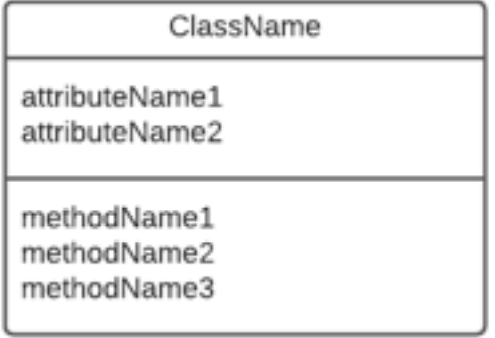
\includegraphics[scale=0.75]{Capture1.PNG}
	%\caption{Légende de l'image}
\end{figure}
\begin{itemize}
	\item[* ] Dans sa forme la plus simple, une classe est représentée comme suit :
	\begin{itemize}
		\item[* ] Un nom (toujours un substantif, au singulier, représente la
		nature des objets de cette classe).
		\item[* ] Une liste d'attributs.
		\item[* ] Une liste de méthodes.
	\end{itemize}
\item[* ] Manque d'informations, mais bon pour un premier tour de table de
conception.
\end{itemize}

\subsection{Encapsulation}
\begin{figure}[!hbtp]
	\centering
	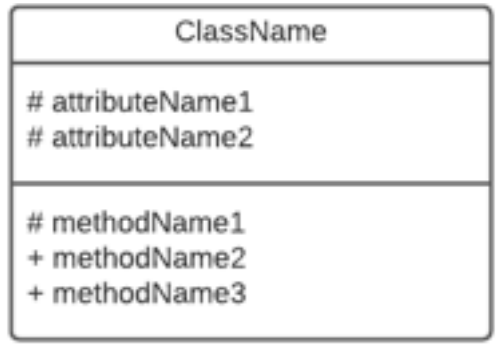
\includegraphics[scale=0.75]{Capture2.PNG}
	%\caption{Légende de l'image}
\end{figure}
\begin{itemize}
	\item[* ] Rappel : définition de l'encapsulation : cacher
	certains attributs ou méthodes à d'autres objets.
	\item[* ] En UML, les éléments peuvent être qualifiés de :
	\begin{itemize}
		\item[* ] public (signe : +) : l'élément n'est pas encapsulé ; visible
		par tout le monde.
		\item[* ] protected (signe : $\sharp$) : l'élément est encapsulé et visible dans les
		visible dans les spécialisations de cette classe.
		\item[* ] private (signe : -) : l'élément est encapsulé (visible uniquement 
		 à l'intérieur de la classe).
		 \item[* ] package (signe : $\sim$) : l'élément est encapsulé et visible à l'intérieur du
		 visible dans le paquetage (nous ne l'utiliserons pas dans cette classe).
	\end{itemize}
\end{itemize}
\subsection{Types}
\begin{figure}[!hbtp]
	\centering
	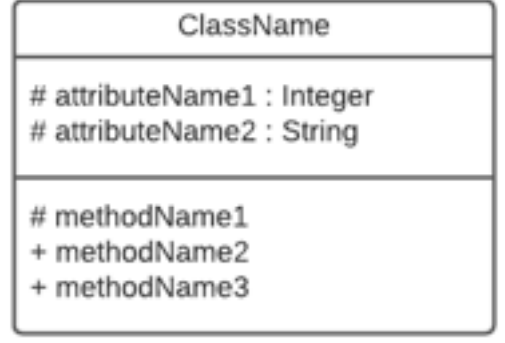
\includegraphics[scale=0.75]{Capture3.PNG}
	%\caption{Légende de l'image}
\end{figure}
\begin{itemize}
	\item[* ] Dans un diagramme de classes, il est possible de spécifier le
	type d'une variable.
	\item[* ] Le type peut être l'un des types standard :
	\begin{itemize}
		\item[* ]  Booléen.
		\item[* ] Entier.
		\item[* ] Réel.
		\item[* ] Chaîne.
		
	\end{itemize}
\item[* ] Ou il peut s'agir d'une classe (du système ou non).
\item[* ] Indiqué par " :" après la variable.

\end{itemize}
\subsection{Valeur par défaut}
\begin{figure}[!hbtp]
	\centering
	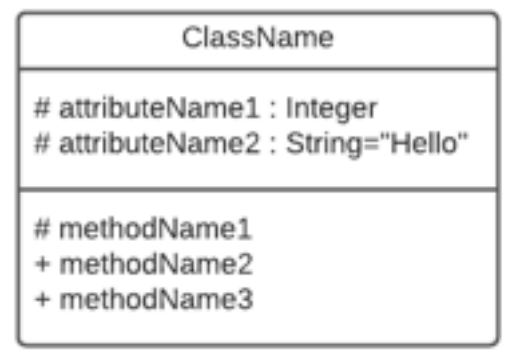
\includegraphics[scale=0.75]{Capture4.PNG}
	%\caption{Légende de l'image}
\end{figure}
\begin{itemize}
	\item[* ] Un attribut de classe peut avoir une valeur par défaut.
	par défaut. Dans ce cas, il sera indiqué par "=".
	valeur par défaut".
\end{itemize}
\subsection{Cardinalité}
\begin{itemize}
	\begin{figure}[!hbtp]
		\centering
		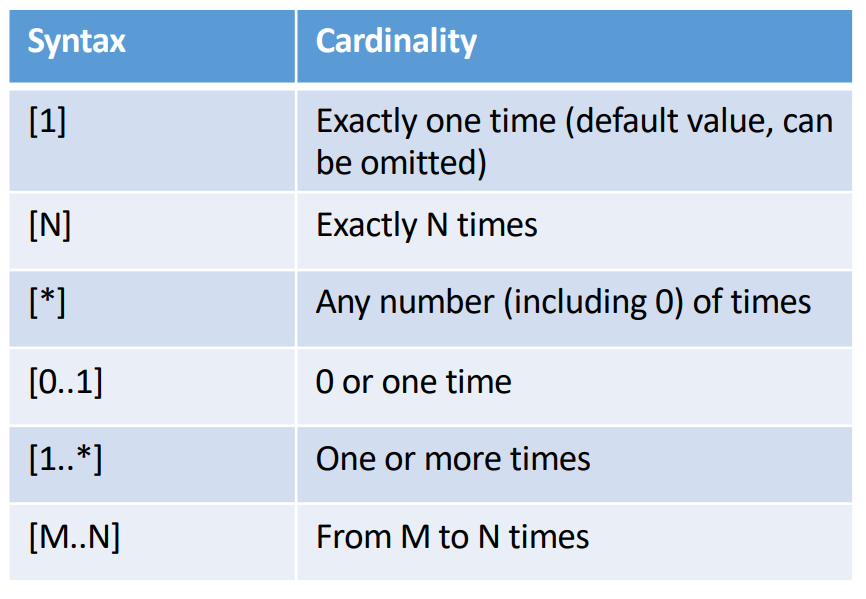
\includegraphics[scale=0.75]{Capture5_1.PNG}
		%\caption{Légende de l'image}
	\end{figure}
	\item[* ] Une variable peut avoir plusieurs valeurs.
	\item[* ] Indiqué par la cardinalité.
	\item[* ] Syntaxe : type [M..N].
	\newpage
	\begin{figure}[!hbtp]
		\centering
		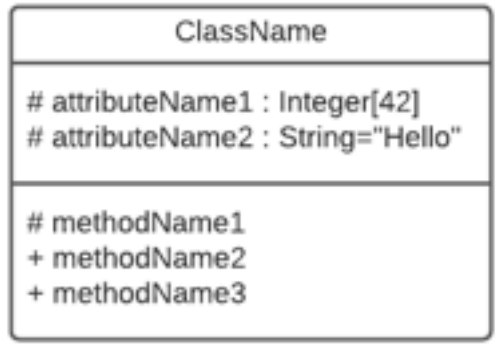
\includegraphics[scale=0.75]{Capture5.PNG}
		%\caption{Légende de l'image}
	\end{figure}
	\item[* ] Dans un langage de programmation, cela serait
	par un tableau, une liste, un vecteur, ...
\end{itemize}
\subsection{Modificateurs}
\begin{itemize}
	\item[* ] Un modificateur peut être utilisé (il est facultatif) pour donner des informations supplémentaires sur une variable.
	\item[* ] Syntaxe {modificateur} ou {m1, m2, ...}.
	\item[* ] Les plus courants :
	\begin{itemize}
		\item[* ] id : la variable fait partie de l'identifiant de la classe
		\item[* ] readOnly : la variable ne peut pas être modifiée.
		\item[* ] rdered (applicable pour les cardinalités > 1) : les valeurs de la variable doivent être ordonnées.
		\item[* ] unique (applicable pour les cardinalités > 1) : les valeurs de la variable doivent être uniques (par défaut !).
		\item[* ] nonunique (applicable pour les cardinalités > 1) : les valeurs de la variable ne doivent pas être uniques.
		\item[* ]  redefines "attribute name" : redéfinition de "attribute name" à partir de la superclasse. Si le type
		est modifié, le nouveau type doit être compatible avec l'ancien type.
	\end{itemize}
\end{itemize}
\subsection{Attributs dérivés}
\begin{figure}[!hbtp]
	\centering
	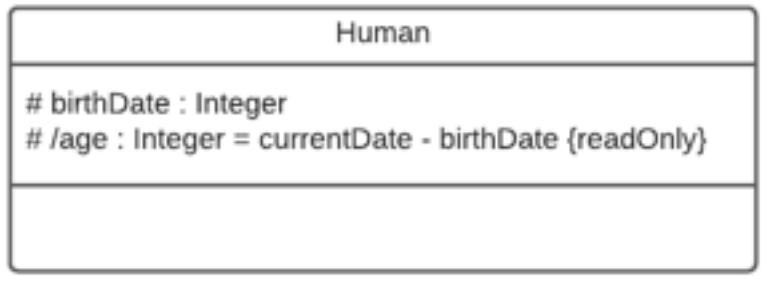
\includegraphics[scale=0.75]{Capture6.PNG}
	%\caption{Légende de l'image}
\end{figure}
\begin{itemize}
	\item[* ] Un attribut peut être dérivé d'autres
	informations (souvent : autre(s) attribut(s)).
	\item[* ] indiqué avec "/" devant le nom.
	\item[* ] Peut être suivi d'une expression expliquant
	comment calculer la valeur.
	\item[* ] Souvent "readOnly" (lecture seule).
\end{itemize}
\subsection{Types 2}
\begin{itemize}
	\item[* ] Pour typer une méthode, nous parlerons de sa "signature" :
	\begin{itemize}
		\item[* ] Nom de la méthode.
		\item[* ] Nom des paramètres, leurs types, leurs cardinalités et propriétés, valeur par défaut.
		\item[* ] Résultat de la méthode : type, cardinalité, propriété.
	\end{itemize}
\item[* ] Syntaxe:\\
\textbf{name (direction nameParam :type[inf..sup]=Default{modifiers}, …) : returnType[inf..sup]\\{modifiers}.}
\item[*] Le sens peut être :
\begin{itemize}
	\item[* ] in : la valeur du paramètre est transmise au moment de l'appel.
	\item[* ] out : la valeur du paramètre est transmise à la fin de l'exécution de la
	méthode.
	\item[* ] inout : les deux.
\end{itemize}

\end{itemize}
\subsection{Attributs dérivés}
\begin{figure}[!hbtp]
	\centering
	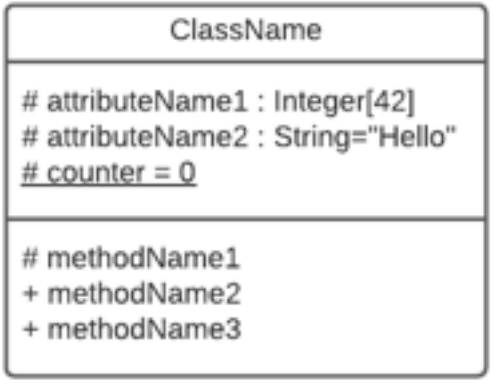
\includegraphics[scale=0.75]{Capture7.PNG}
	%\caption{Légende de l'image}
\end{figure}
\begin{itemize}
	\item[* ] Une instance d'une classe = une instance de chaque
	attribut.
	\item[* ] Il est possible d'avoir des attributs qui sont liés
	à la classe plutôt qu'à une instance. Dans ce
	cas, on parlera d'"attributs de classe".
	\item[* ] Un attribut de classe est le même (nom, valeur,
	type) pour chaque instance. En général, il doit
	avoir une valeur par défaut.
	\item[* ] Un attribut de classe n'est jamais hérité.
	\item[* ] On y accède par la classe directement (pas par une
	instance).
	\item[* ] Syntaxe : soulignez l'attribut.
\end{itemize}
\subsection{Méthodes de classe}
\newpage
\begin{figure}[!hbtp]
	\centering
	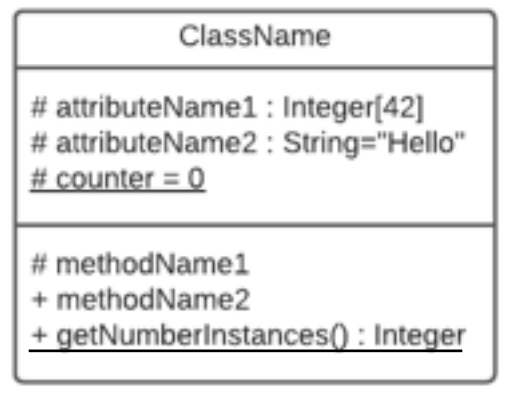
\includegraphics[scale=0.75]{Capture8.PNG}
	%\caption{Légende de l'image}
\end{figure}
\begin{itemize}
	\item[* ] De même, une méthode peut être liée à une classe, auquel cas nous parlerons de "méthode de classe".
	auquel cas on parlera de "méthode de classe".
	\item[* ] ne peut être accédée que par la classe elle-même
	et ne peut utiliser que les attributs de la classe.
\end{itemize}
\subsection{Représenter une classe - récapitulation}
\begin{figure}[!hbtp]
	\centering
	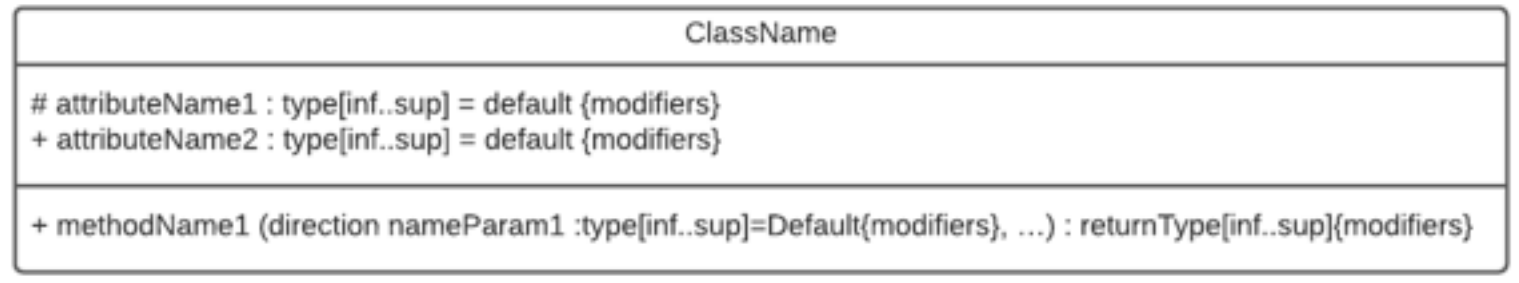
\includegraphics[scale=0.75]{Capture9.PNG}
	%\caption{Légende de l'image}
\end{figure}
\subsection{Association entre les classes}
\begin{itemize}
	\begin{figure}[!hbtp]
		\centering
		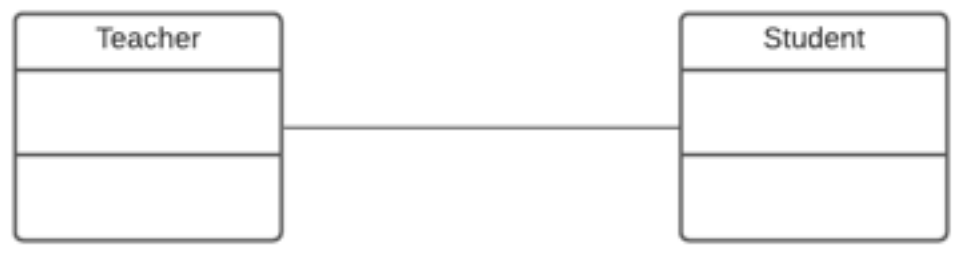
\includegraphics[scale=0.75]{Capture10.PNG}
		%\caption{Légende de l'image}
	\end{figure}
	\item[* ] Une association peut être établie entre
	deux (ou plusieurs) classes qui sont reliées.
	\item[* ] Montre comment les classes sont liées à travers le
	système.
	\item[* ] Syntaxe ligne pleine (pour les relations binaires).
	\newpage
	\begin{figure}[!hbtp]
		\centering
		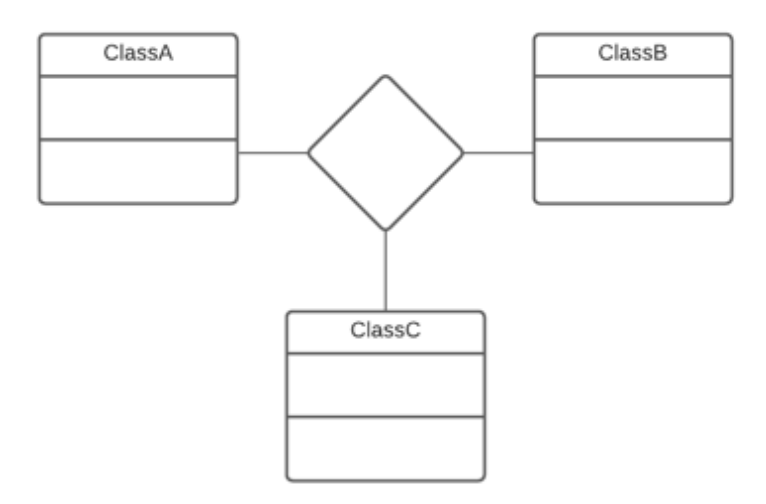
\includegraphics[scale=0.75]{Capture11.PNG}
		%\caption{Légende de l'image}
	\end{figure}
	\item[* ] Relations ternaires (ou N-aires) : avec un losange.
	\begin{figure}[!hbtp]
		\centering
		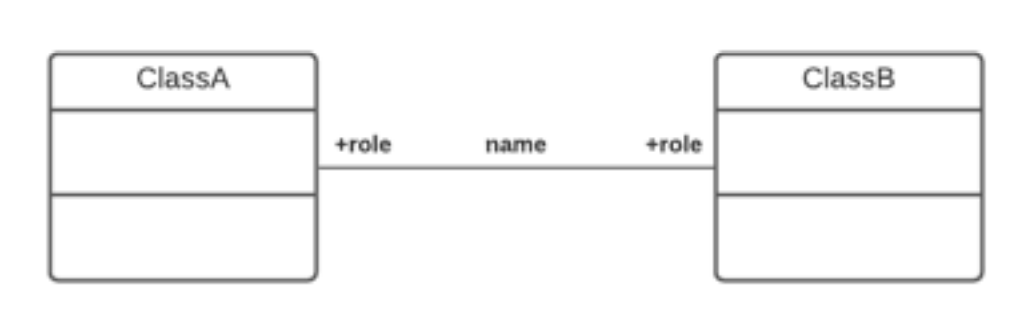
\includegraphics[scale=0.75]{Capture12.PNG}
		%\caption{Légende de l'image}
	\end{figure}
	\item[* ]  L'association peut être nommée.
	\item[* ] Le rôle de chaque instance peut être indiqué avec la syntaxe "+role".
\end{itemize}
\subsection{Cardinalité}
\begin{itemize}
	\item[* ] Possibilité d'ajouter la cardinalité aux associations.
	\item[* ] La cardinalité sur le côté d'une classe indique combien d'instances de cette classe sont liées à une instance de la classe à l'autre extrémité.
	\item[* ] Exemple : 1 à 3 instances de ClassA sont liées à chaque instance de ClassB.
 0 instance ou plus de ClassB est liée à chaque instance de
	ClasseA
		\begin{figure}[!hbtp]
		\centering
		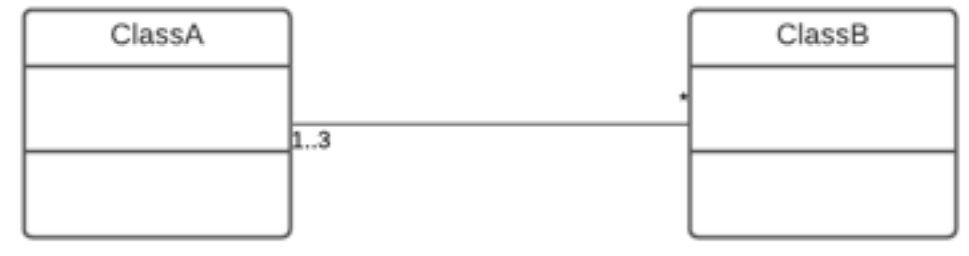
\includegraphics[scale=0.75]{Capture13.PNG}
		%\caption{Légende de l'image}
	\end{figure}
\end{itemize}
\subsection{Composition}
\begin{itemize}
	\item[* ] Rappel : Composition : les objets complexes peuvent être composés d'autres
	objets.
	\item[* ] Elle est définie au niveau de la classe, mais on ne compose que des instances réelles.
	\item[* ] Elle peut être :
	\begin{itemize}
		\item[* ] une relation forte : les composants ne peuvent pas être partagés ; la destruction de l'objet composé implique la destruction des composants.
		l'objet composé implique la destruction des composants
		\item[* ] une relation faible (aussi appelée agrégation) : les composants peuvent être partagés.
	
	\end{itemize}
	\item[* ] Une composition est une association !
\item[* ] Relation "a".
\end{itemize}
\subsection{Composition forte (a.k.a. composition)}
\begin{itemize}
	\item[* ] Composition forte : les composants
	ne peuvent pas être partagés -> la cardinalité du
	côté de la composition est toujours 1.
		\begin{figure}[!hbtp]
		\centering
		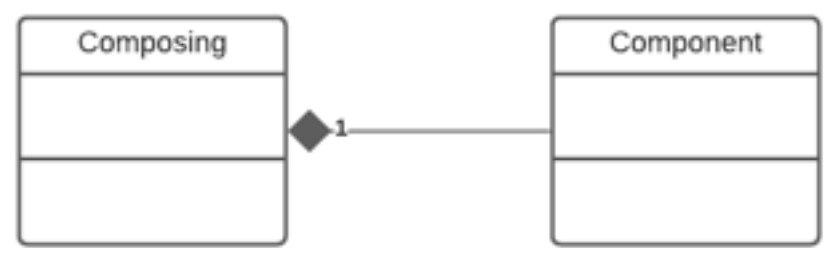
\includegraphics[scale=0.75]{Capture14.PNG}
		%\caption{Légende de l'image}
	\end{figure}
\item[* ] Exemple : une instance d'un humain a
un cerveau et au plus 2 bras.
	\begin{figure}[!hbtp]
	\centering
	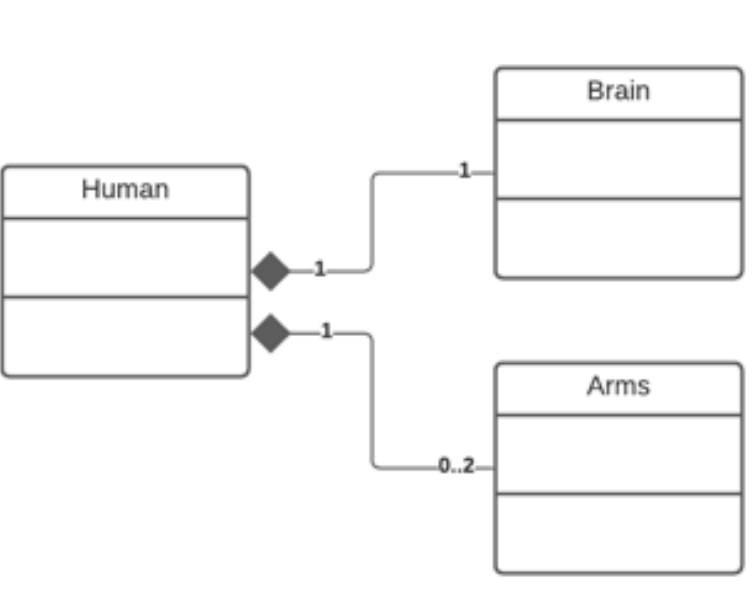
\includegraphics[scale=0.75]{Capture15.PNG}
	%\caption{Légende de l'image}
\end{figure}
\end{itemize}
\subsection{Composition faible (alias agrégation)}
\begin{itemize}
	\item[* ] Composition faible : les composants peuvent être partagés et la destruction de l'objet
	l'objet qui compose ne détruit pas le composant.
	\item[* ]  Plus fréquente que la composition forte.
	\newpage
		\begin{figure}[!hbtp]
		\centering
		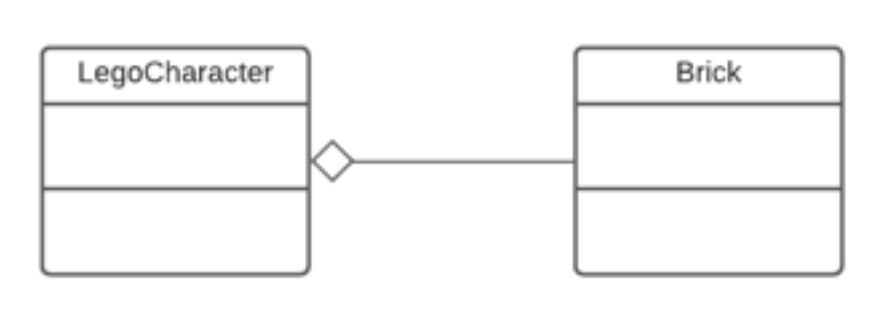
\includegraphics[scale=0.75]{Capture16.PNG}
		%\caption{Légende de l'image}
	\end{figure}
\end{itemize}
\subsection{Directionalité}
\begin{itemize}
	\item[* ] Par défaut, les associations sont bidirectionnelles : à partir d'une instance de
	classeA, je devrais pouvoir trouver le lien vers la classeB et à partir d'une instance de la classeB, je devrais pouvoir trouver le lien vers la classeA.
	et à partir d'une instance de ClassB, je devrais être capable de trouver le lien vers ClassA.
	\item[* ]  En général, pas bon en pratique.
	\item[* ] Possibilité d'ajouter une flèche pour indiquer le sens de l'association.
	\item[* ] Exemple : ClassA sait qu'elle est liée à ClassB, mais ClassB ne le sait pas.
		\begin{figure}[!hbtp]
		\centering
		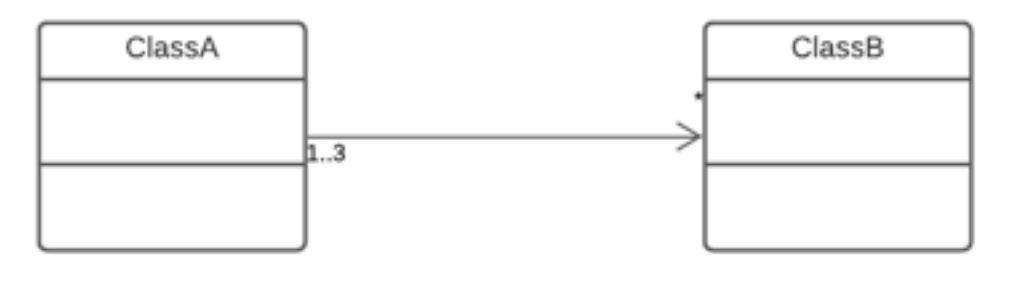
\includegraphics[scale=0.75]{Capture17.PNG}
		%\caption{Légende de l'image}
	\end{figure}
\end{itemize}
\subsection{Association réflexive}
\begin{itemize}
	\item[* ] Il est possible d'avoir une association d'une classe à elle-même.
	\item[* ] Peut être utilisé pour créer:
	\begin{itemize}
		\item[* ] une hiérarchie.
		\item[* ] un groupe.
	\end{itemize}
	\begin{figure}[!hbtp]
	\centering
	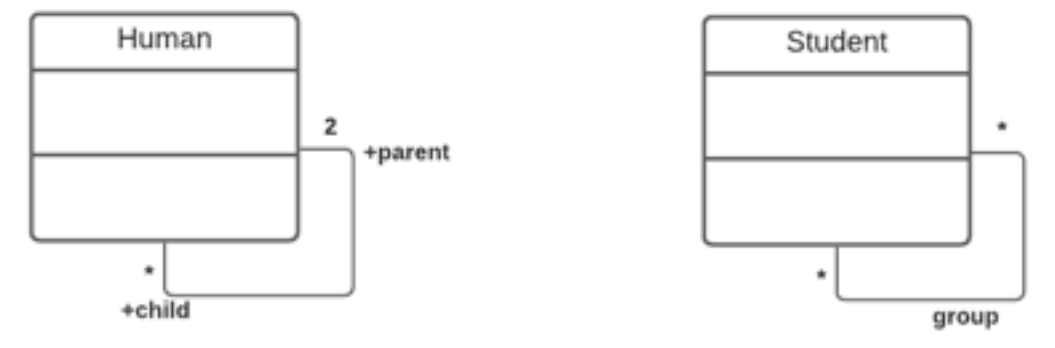
\includegraphics[scale=0.75]{Capture18.PNG}
	%\caption{Légende de l'image}
\end{figure}
\end{itemize}
\subsection{Classes d'association}
\begin{itemize}
	\item[* ] Dans certains cas, l'association peut être complexe.
	\item[* ] Dans ce cas, l'association peut être modélisée comme une classe.
	\item[* ] Syntaxe : ligne en pointillé entre la classe d'association et la classe de
	association.
	\item[* ] Exemple:
	\begin{figure}[!hbtp]
		\centering
		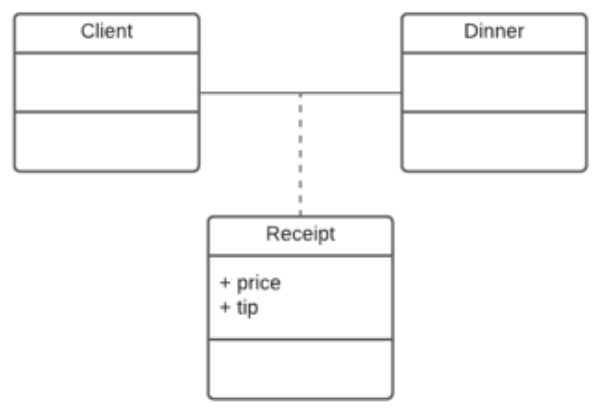
\includegraphics[scale=0.75]{Capture19.PNG}
		%\caption{Légende de l'image}
	\end{figure}
\end{itemize}
\subsection{Association de dépendance}
\begin{itemize}
	\item[* ]  Association dirigée.
	\item[* ] Indique qu'une classe a besoin d'une autre classe pour sa spécification ou son
	implémentation.
	\item[* ] Syntaxe:
	\begin{figure}[!hbtp]
		\centering
		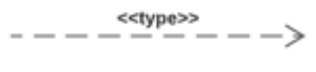
\includegraphics[scale=0.75]{Capture20.PNG}
		%\caption{Légende de l'image}
	\end{figure}
\item[* ] Le type indique la dépendance et peut être :
\begin{itemize}
	\item[* ] call : utilise une méthode.
	\item[* ] create : crée une instance.
	\item[* ] derive : indique une redondance.
	\item[* ] instantiate : classe d'usine qui a besoin de cette autre classe pour sa spécification.
	\item[* ] permit : permet l'accès à des éléments privés.
	\item[* ] use : cas général.
	\item[* ] Exemple : la classe ChocolateFactory est une usine qui a pour seul objectif de produire (instancier) des instances de barres de chocolat.
	but de produire (instancier) des instances de ChocolateBar.
	La ChocolateFactory a donc besoin de connaître la spécification de la
	barre chocolatée pour la produire.
	\newpage
		\begin{figure}[!hbtp]
		\centering
		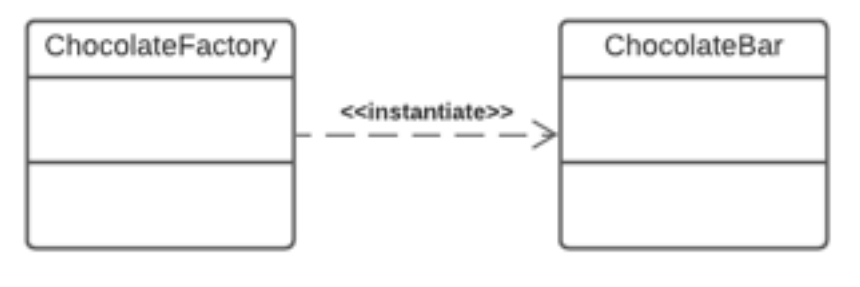
\includegraphics[scale=0.75]{Capture21.PNG}
		%\caption{Légende de l'image}
	\end{figure}
\end{itemize}
\end{itemize}
\subsection{Associations - récapitulation}
\begin{itemize}
	\item[* ] Une association entre deux classes représente un lien entre
	elles.
	\item[* ] Dans le cas général, l'association est qualifiée par des noms et des rôles
	et indique un lien simple entre les classes (trait plein).
	\item[* ] Composition : indique un composant qui ne peut pas être partagé.
	\item[* ] Agrégation : indique un composant qui peut être partagé.
	\item[* ] Flèche pointillée : dépendance entre classes.
\end{itemize}
\subsection{Généralisation/spécialisation : rappel}
\begin{itemize}
	\item[* ]  Spécialisation : une nouvelle classe A peut être créée en tant que sous-classe d'une autre classe B. Dans ce cas, la classe A spécialise la classe B.
	\item [* ] La spécialisation est une relation "est un".
	\item[* ] La généralisation est l'inverse (la superclasse B est une généralisation de la sous-classe A).
	sous-classe A).
	\item[* ] Héritage : le fait qu'une sous-classe obtienne le comportement et la
	structure de la superclasse.
	\item[* ]  C'est une conséquence de la spécialisation.
	\item[* ] Syntaxe:
		\begin{figure}[!hbtp]
		\centering
		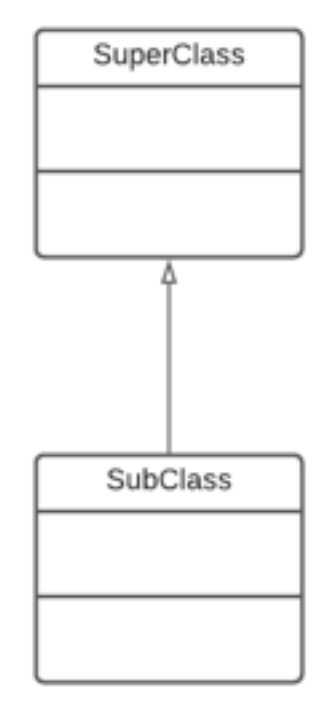
\includegraphics[scale=0.75]{Capture22.PNG}
		%\caption{Légende de l'image}
	\end{figure}
\end{itemize}

\end{document}